\documentclass[12pt]{article}
\usepackage[english]{babel}
\usepackage[utf8x]{inputenc}
\usepackage{amsmath}
\usepackage{graphicx}
\usepackage{hyperref, url}
\usepackage[colorinlistoftodos]{todonotes}
\usepackage[font=small,labelfont=bf]{caption}

\begin{document}
	
	\begin{titlepage}
		
		\newcommand{\HRule}{\rule{\linewidth}{0.5mm}} % Defines a new command for the horizontal lines, change thickness here
		
		\center % Center everything on the page
		
		%----------------------------------------------------------------------------------------
		%	HEADING SECTIONS
		%----------------------------------------------------------------------------------------
		
		\textsc{\LARGE Central Washington University}\\[1.5cm] % Name of your university/college
		\textsc{\Large High Performance Computing}\\[0.5cm] % Major heading such as course name
		\textsc{\large Spring 2019}\\[0.5cm] % Minor heading such as course title
		
		%----------------------------------------------------------------------------------------
		%	TITLE SECTION
		%----------------------------------------------------------------------------------------
		
		\HRule \\[0.4cm]
		{ \huge \bfseries Image Classification Using Keras}\\[0.4cm] % Title of your document
		\HRule \\[1.5cm]
		
		%----------------------------------------------------------------------------------------
		%	AUTHOR SECTION
		%----------------------------------------------------------------------------------------
		
		\begin{minipage}{0.4\textwidth}
			\begin{flushleft} \large
				\emph{Author:}\\
				Hermann \textsc{Yepdjio} % Your name
			\end{flushleft}
		\end{minipage}
		~
		\begin{minipage}{0.4\textwidth}
			\begin{flushright} \large
				\emph{Supervisor:} \\
				Dr. Szilard \textsc{Vajda} % Supervisor's Name
			\end{flushright}
		\end{minipage}\\[0.2cm]
		
		% If you don't want a supervisor, uncomment the two lines below and remove the section above
		%\Large \emph{Author:}\\
		%John \textsc{Smith}\\[3cm] % Your name
		
		%----------------------------------------------------------------------------------------
		%	DATE SECTION
		%----------------------------------------------------------------------------------------
		
		{\large \today}\\ % Date, change the \today to a set date if you want to be precise
		
		%----------------------------------------------------------------------------------------
		%	LOGO SECTION
		%----------------------------------------------------------------------------------------
		
		
\includegraphics[width=12cm]{CWU-Logo.png}\\[.5cm] % Include a department/university logo - this will require the graphicx package
		
		%----------------------------------------------------------------------------------------
		
		\vfill % Fill the rest of the page with whitespace
		
	\end{titlepage}
	\newpage
	\tableofcontents
	\newpage
	
	
	
	\section{Introduction}
		Project 3 was about classifying images using Keras and Tensorflow. The goal was to run some experiments, changing some parameters each time or increasing the number of hidden layers in the network in order to improve the classification accuracy of the model. The data set used in this project to train and test the model as well as the python code used to create the initial model were obtained from \cite{1}. The code was modified to adjust the parameters and add more layers to the network, and the resulting models were evaluated for the classification accuracy. The results of the experiments are discussed in the following section.
		
	\section{Results for Experimentation Using Training and Testing Sets}
		\subsection{Increasing the Number of Convolution Layers and the Number of Epochs}
		
			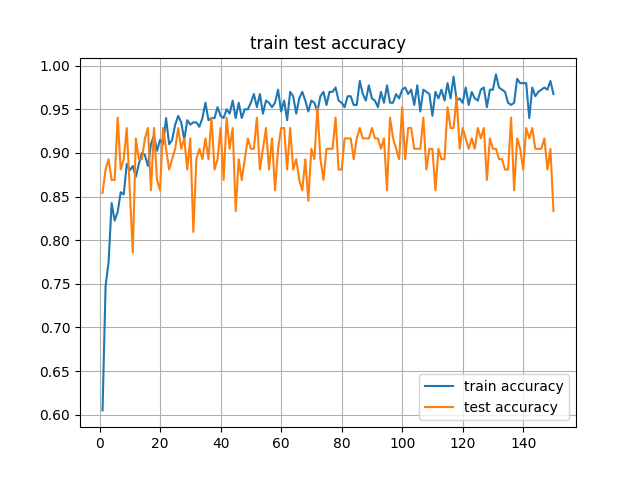
\includegraphics[width=\linewidth - 2cm]{accuracy_2_hidden_layers.png}
			\captionof{figure}{Accuracy Vs Epoch for a Network with Three Convolution Layers}	
			
			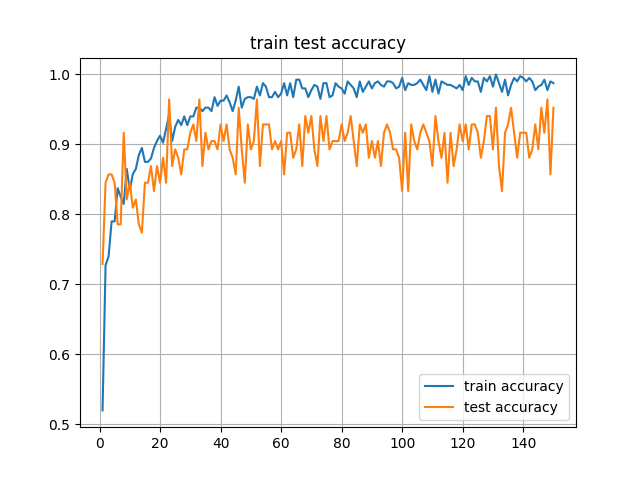
\includegraphics[width=\linewidth - 2cm]{accuracy_4_hidden_layers.png}
			\captionof{figure}{Accuracy Vs Epoch for a Network with Five Convolution Layers}	
			
			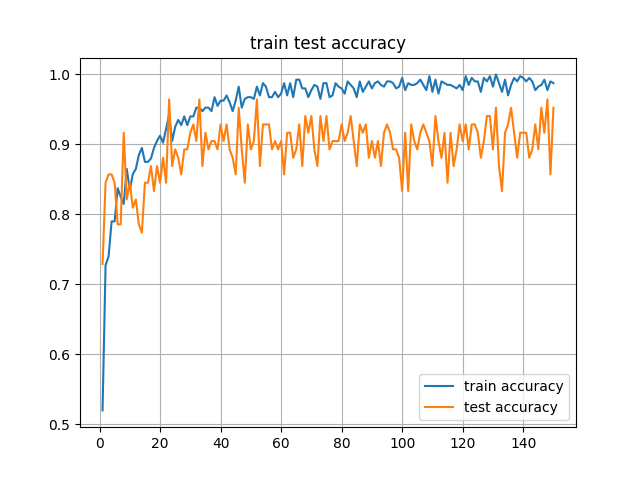
\includegraphics[width=\linewidth - 2cm]{accuracy_4_hidden_layers.png}
			\captionof{figure}{Accuracy Vs Epoch for a Network with Seven Convolution Layers}	
			
			As figures 1, 2 and 3 above show, the train classification accuracy tends to increase as the epoch number increases while the test classification accuracy pretty much remains stable (between .75 and .95). Those figures also show that the train classification accuracy improves as the number of convolution layers increases.
			
		\subsection{Increasing the Batch Size and the Number of Epochs}
			
			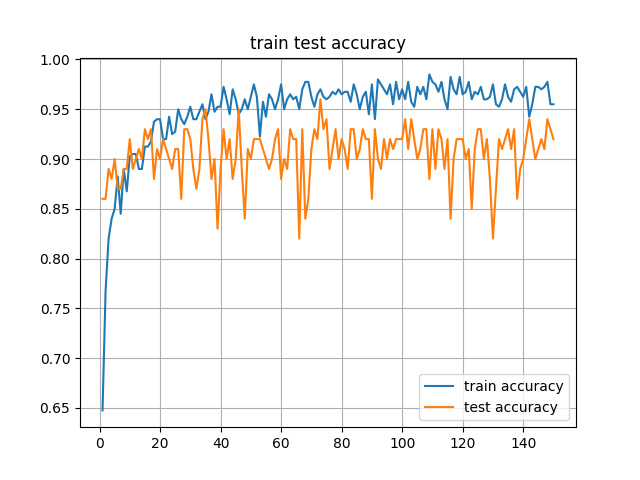
\includegraphics[width=\linewidth - 2cm]{accuracy_2_hl_10.png}
			\captionof{figure}{Accuracy Vs Epoch with Batch Size = 10}	
			
			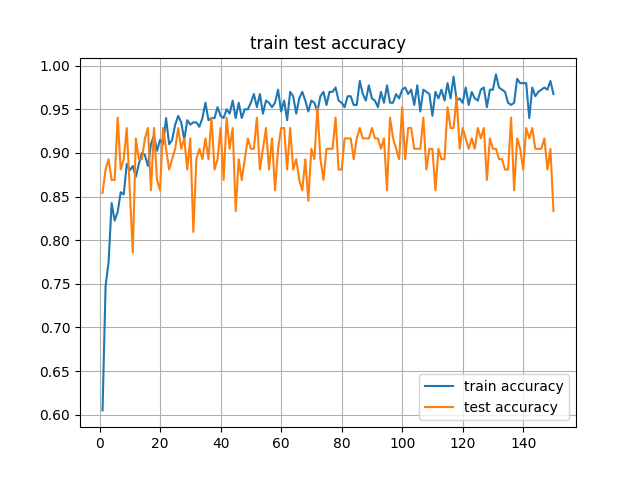
\includegraphics[width=\linewidth - 2cm]{accuracy_2_hidden_layers.png}
			\captionof{figure}{Accuracy Vs Epoch with Batch Size = 16}	
			
			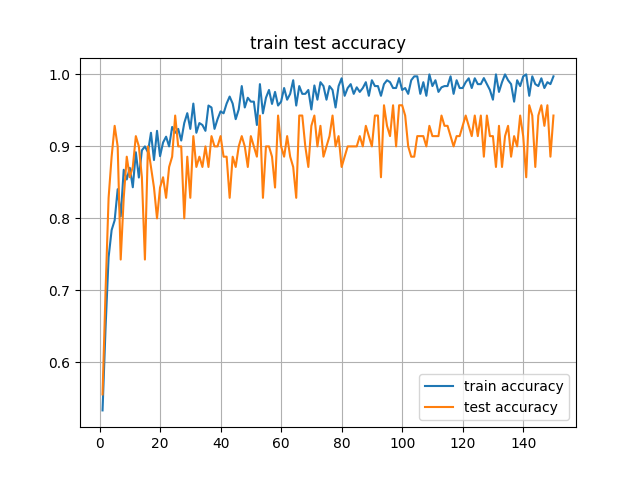
\includegraphics[width=\linewidth - 2cm]{accuracy_2_hl_30.png}
			\captionof{figure}{Accuracy Vs Epoch with Batch Size = 30}
			
			The patterns seen in section 2.1 can be observed in figures 4, 5, and 6 as well. That is, the train classification accuracy tends to increase as the epoch number increases while the test classification accuracy remains stable (between .75 and .95) and the train classification accuracy improves as the 
			batch size increases.
	\section{Result of Experimentation Using Ten Folds Cross Validation}
	
		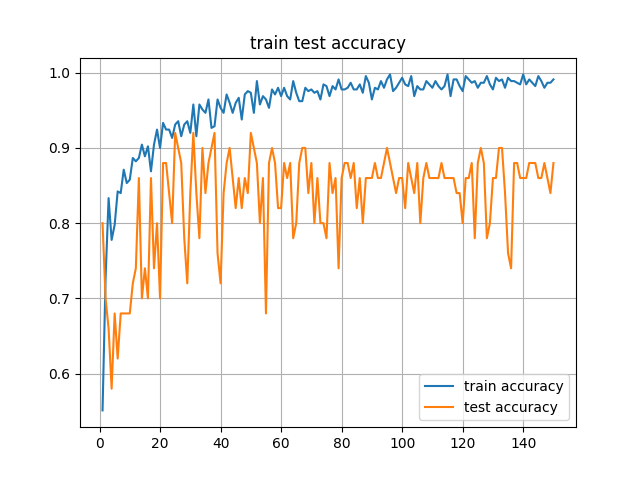
\includegraphics[width=\linewidth - 2cm]{accuracy_fold0.png}
		\captionof{figure}{Accuracy Vs Epoch for Fold 1}
		
		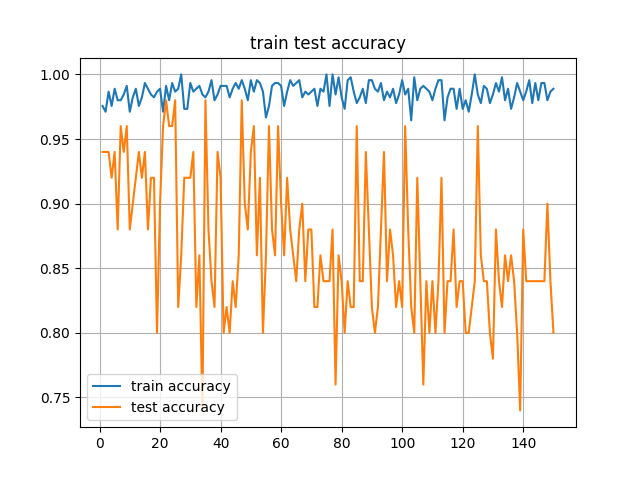
\includegraphics[width=\linewidth - 2cm]{accuracy_fold1.png}
		\captionof{figure}{Accuracy Vs Epoch for Fold 2}
		
		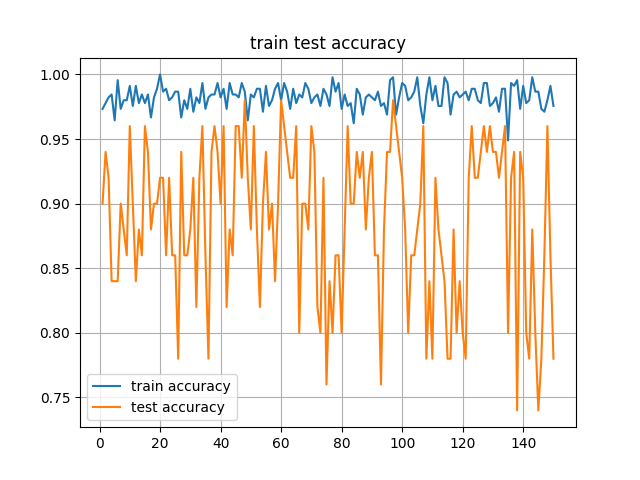
\includegraphics[width=\linewidth - 2cm]{accuracy_fold2.png}
		\captionof{figure}{Accuracy Vs Epoch for Fold 3}
		
		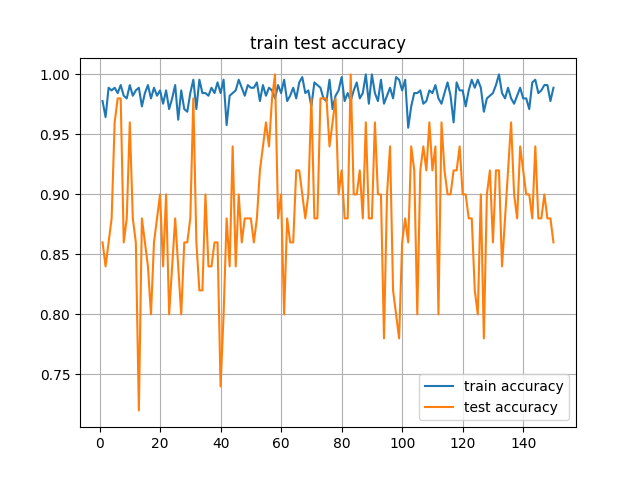
\includegraphics[width=\linewidth - 2cm]{accuracy_fold3.png}
		\captionof{figure}{Accuracy Vs Epoch for Fold 4}
		
		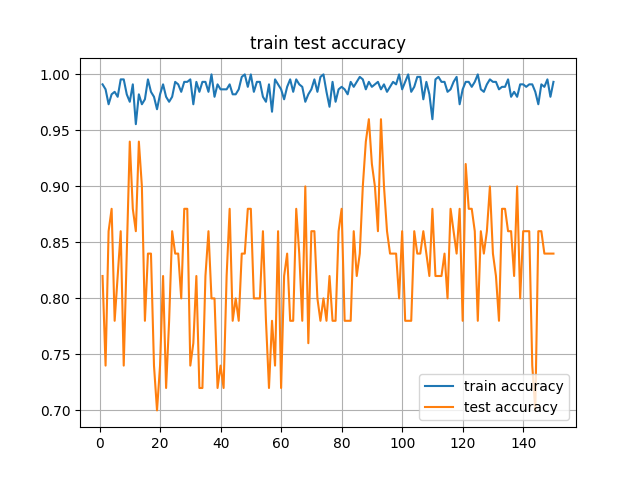
\includegraphics[width=\linewidth - 2cm]{accuracy_fold4.png}
		\captionof{figure}{Accuracy Vs Epoch for Fold 5}
		
		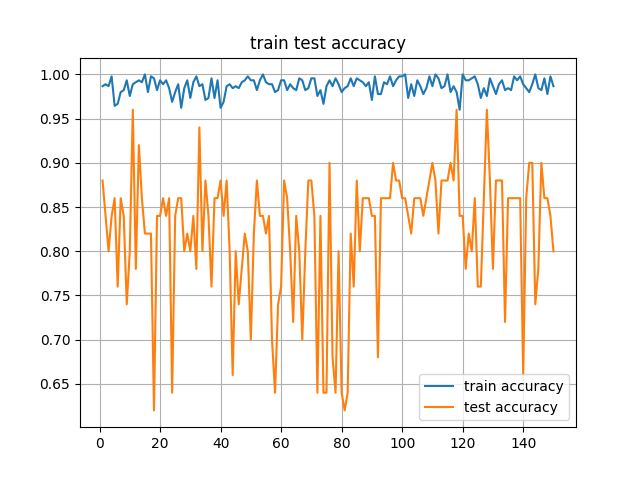
\includegraphics[width=\linewidth - 2cm]{accuracy_fold5.png}
		\captionof{figure}{Accuracy Vs Epoch for Fold 6}
		
		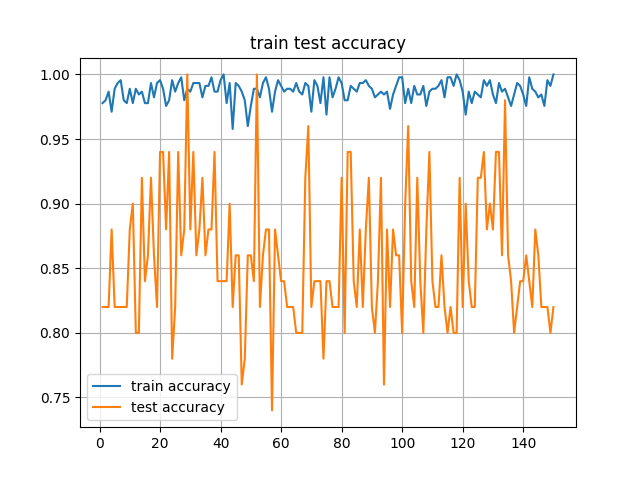
\includegraphics[width=\linewidth - 2cm]{accuracy_fold6.png}
		\captionof{figure}{Accuracy Vs Epoch for Fold 7}
		
		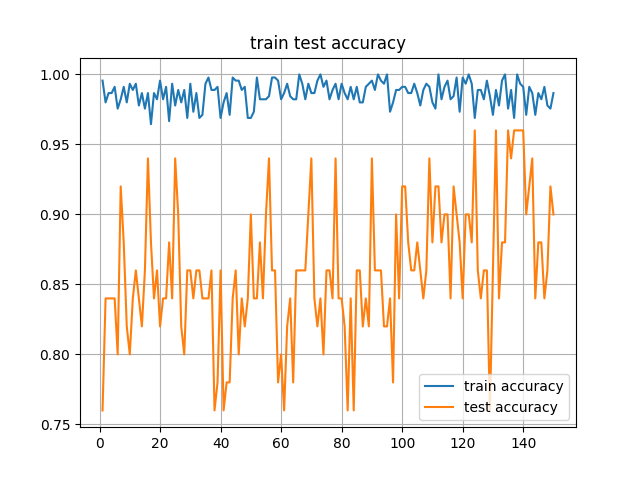
\includegraphics[width=\linewidth - 2cm]{accuracy_fold7.png}
		\captionof{figure}{Accuracy Vs Epoch for Fold 8}
		
		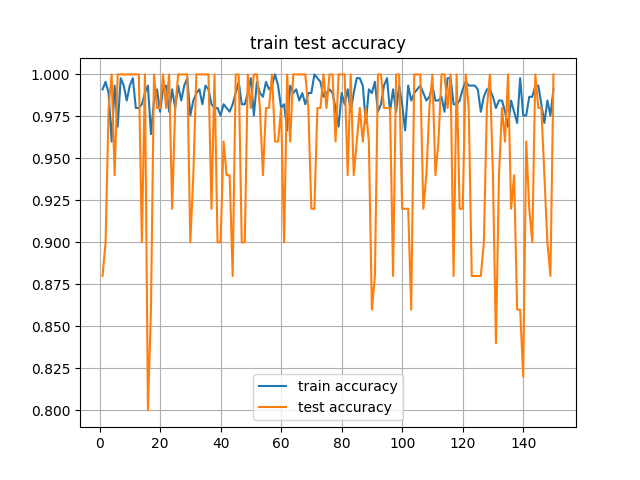
\includegraphics[width=\linewidth - 2cm]{accuracy_fold8.png}
		\captionof{figure}{Accuracy Vs Epoch for Fold 9}
		
		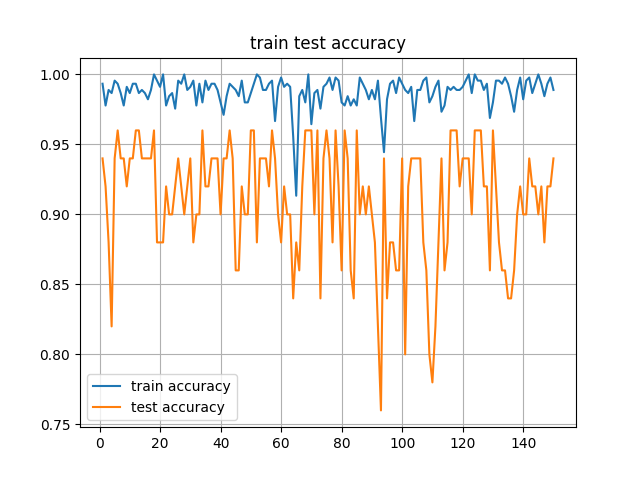
\includegraphics[width=\linewidth - 2cm]{accuracy_fold9.png}
		\captionof{figure}{Accuracy Vs Epoch for Fold 10}
		
		Figures 7 show that both the train and test classification accuracies increase as the number of epochs increases for Fold 1. However, figures 8 - 16 show that the train classification accurancy remain stable (between .90 and 1) while the test classification accuracy is really unstable (varies between .62 and 1). Figure 15 show that fold 9 has the most unstable test classification accuracy across the epochs as it varies between .6 and 1.
	
	\section{Conclusion}
		The experiments ran in project 3 show that changing the configuration of a network can affect its outcome in good or in bad. Increasing the number of convolution layers or the batch size did not really affect the test classification accuracy. However, using 10 folds cross validation produced the highest test classification accuracy (which was 1 according to Figure 15) for fold 9, but overall it also produced the most unstable classification accuracy across the epochs.
	
		
	\begin{thebibliography}{1}
		
		\bibitem{1} NitishGangwar, \textit{Python|Image Classification using keras} \url{https://www.geeksforgeeks.org/python-image-classification-using-keras/}
			\end{thebibliography}
\end{document}